\documentclass[12pt,twocolumn]{article}
\usepackage[margin=1.5cm]{geometry}
\usepackage{amsmath}
\usepackage{graphicx}
\usepackage{hyperref}
\title{Properties of Concave Lenses}
\author{Prof. Jordan C. Hanson}

\begin{document}
\small
\maketitle

\section{Introduction}

\noindent
In this activity, we will verify the \textit{thin lens equations}:

\begin{align}
\frac{1}{d_{\rm o}} + \frac{1}{d_{\rm i}} =& \frac{1}{f} \label{eq:f} \\
m = \frac{h_{\rm i}}{h_{\rm o}} =& -\frac{d_{\rm i}}{d_{\rm o}}  \label{eq:m}
\end{align}

In Eq. \ref{eq:f}, $d_{\rm o}$ is the distance between the object and the lens origin, and $d_{\rm i}$ is the distance to the image.  In this lab activity, we will use a concave lens with a focal length $f$ that produces real images.  The parameter $m$ is called the magnification, representing the ratio of image height $h_{\rm i}$ to object height $h_{\rm o}$.

We will verify Eq. \ref{eq:f} by varying $d_{\rm o}$ with respect to the lens origin and measuring $d_{\rm i}$.  The value of $d_{\rm i}$ corresponds to the distance from lens origin at which the real image is in focus. The focal length $f$ is a constant in this experiment.  Thus, the only measurement required to verify Eq. \ref{eq:f} is $d_{\rm i}$.  To verify Eq. \ref{eq:m}, we will confirm two facts.  First, we will confirm that the focused image is inverted and that $d_{\rm i}>0$, which will justify the minus sign in Eq. \ref{eq:m}.  Second, we will measure $m$ geometrically, and verify that this matches $d_{\rm i}/d_{\rm o}$.

\section{Experimental Setup}

\begin{figure}[ht]
\centering
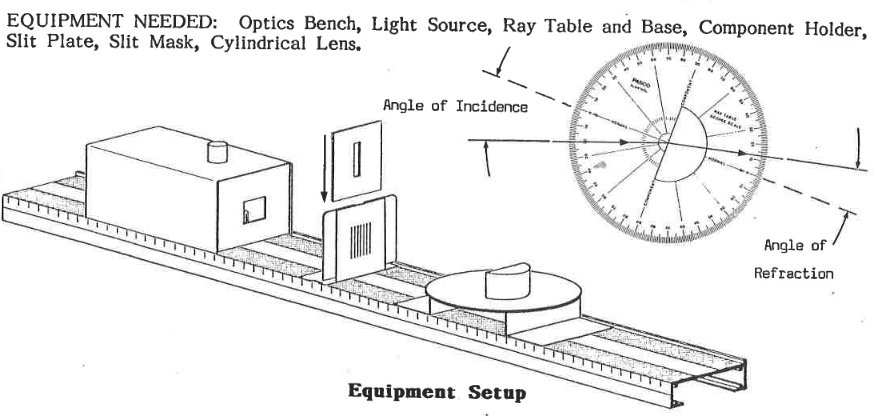
\includegraphics[width=0.49\textwidth,trim=0cm 0cm 0cm 2cm,clip=true]{equip.png}
\caption{\label{fig:equip} A diagram of the setup.}
\end{figure}

\noindent
The procedure depicted in Fig. \ref{fig:equip} should produce results that verify Eqs. \ref{eq:f} and \ref{eq:m}.  Check that you have the following items at your table:

\begin{itemize}
\item Optics bench
\item Light source
\item Magnetic object holder with crossed-arrow target
\item Magnetic object holder with concave lens ($f = 75$ mm or $f=150$ mm)
\item Magnetic object holder with viewing screen
\item Meter stick
\end{itemize}

Place the light source as far as possible at one end of the optics bench.  Plus the crossed arrow target in front of the light source using the magnetic holder.  Using another magnetic holder, place the concave lens more than one focal length away from the target.  The designed focal length is written on the lens, and we will verify this constant with our measurements.  Finally, place the viewing screen more than one focal length from the lens origin, using a magnetic holder.  Plug in the light source, and turn it on.  Adjust the primary ray direction with the knob on the top of the light source as necessary.  Move the viewing screen forwards and backwards until a focused image forms on it.  Now orient the system such that $d_{\rm o}$ is as large as possible, and $d_{\rm i}$ is as close to one focal length $f$ away from the lens.

\section{Data Analysis for Eq. \ref{eq:f}}

\noindent
Complete Tab. \ref{tab:data} below, filling in the numbers appropriately.  The idea is to vary $d_{\rm o}$, and quote the value in both mm and factors of $f$.  For example, if $f = 150$ mm, and $d_{\rm o} = 75$ mm, then $d_{\rm o}/f = 0.5$.  Since $f$ is the natural unit of distance for the lens, it is a good idea to measure $d_{\rm i}$ for a variety of values of $d_{\rm o}/f$.  Do not worry if you cannot obtain a focused image for every table entry.  Notice that if multiply both side of Eq. \ref{eq:f} by $f$, we find

\begin{equation}
\frac{f}{d_{\rm o}} + \frac{f}{d_{\rm i}} = 1
\end{equation}

\begin{table}[ht]
\footnotesize
\centering
\begin{tabular}{| c | c | c | c | c |}
\hline
\textbf{$d_{\rm o}$ [mm]} & \textbf{$d_{\rm o}/f$} & \textbf{$d_{\rm i}$ [mm]} & \textbf{$d_{\rm i}/f$} & $f/d_{\rm o} + f/d_{\rm i}$\\ \hline
 & 2.0 & & & \\ \hline
 & 1.9 & & & \\ \hline
 & 1.8 & & & \\ \hline
 & 1.7 & & & \\ \hline
 & 1.6 & & & \\ \hline
 & 1.5 & & & \\ \hline
 & 1.4 & & & \\ \hline
 & 1.3 & & & \\ \hline
 & 1.2 & & & \\ \hline
 & 1.1 & & & \\ \hline \hline
\textbf{Average:} & -- & -- & -- & \\ \hline
\end{tabular}
\caption{\label{tab:data} Perform the necessary measurements to complete this table.}
\end{table}

To complete the entries in Tab. \ref{tab:data}, it is convenient to use a spreadsheet in Excel or Google Sheets at your table.  Manipulate the data to fill in the sum of ratios in the fifth column of Tab. \ref{tab:data}, and compute the average and standard deviation.  Quote your result in the following format: $1.1 \pm 0.1$.  Is your result consistent with 1.0?  Why or why not?

\section{Data Analysis for Eq. \ref{eq:m}}

To verify Eq. \ref{eq:m}, we must compare the ratio $-d_{\rm i}/d_{\rm o}$ to the \textit{measured} value of $m$.  First, note that each focused image must be inverted relative to the target to qualify as a negative magnification.  Second, note that we are \textit{measuring} $m$ by using the ruler on the target screen, and comparing to the \textit{measured} ratio $-d_{\rm i}/d_{\rm o}$.  The measured $m$ value is the ratio of the length the image arrow to the original arrow (see Eq. \ref{eq:m}).  Quote the average and standard deviation of the difference in the final row of Tab. \ref{tab:data2} in the following format: $0.02 \pm 0.02$.  Are your results consistent with zero?  Why or why not?

\begin{table}[hb]
\footnotesize
\centering
\begin{tabular}{| c | c | c | c | c |}
\hline
\textbf{$d_{\rm o}$ [mm]} & \textbf{$d_{\rm i}$ [mm]} & \textbf{$m_{\rm meas}$} & \textbf{$-d_{\rm i}/d_{\rm o}$} & \textbf{Difference} \\ \hline
 & & & & \\ \hline
 & & & & \\ \hline
 & & & & \\ \hline
 & & & & \\ \hline
 & & & & \\ \hline
 & & & & \\ \hline
 & & & & \\ \hline
 & & & & \\ \hline
 & & & & \\ \hline
 & & & & \\ \hline \hline
 \textbf{Average:} & -- & -- & -- & \\ \hline
\end{tabular}
\caption{\label{tab:data2} Import your data from Tab. \ref{tab:data} here to test Eq. \ref{eq:m}.  In the final column enter the difference between $m_{\rm meas}$ and $-d_{\rm i}/d_{\rm o}$.}
\end{table}

\end{document}